\chapter{Définitions générales sur les courbes elliptiques}
\begin{center}
    Dans ce chapitre, on donne d'abord la définition générale d'une courbe elliptique. On fais
    le lien entre cette définition et la définition qui utilise une forme simplifié de
    l'équation général. On propose également un lemme qui permet de caractériser simplement les courbes
    non-lisses. Finalement, on donne la définition d'un points rationnels d'une courbe
    elliptique.
\end{center}

\section{Définition générale}

La définition générale d'une courbe elliptique est la suivante
\begin{definition}
    Soient $K$ un corps, $\overline{K}$ sa cloture algébrique, et $K^{*}$ son groupe
    multiplicatif. Une courbe elliptique sur $K$ est une cubique, non singulière,
    définie comme l'ensemble des solutions du plan projectif $\mathbb{P}_{2}(\overline{K})$ de
    l'équation de Weierstrass homogène suivante:

\begin{align}
\label{eq:geneEll}
E: Y^2Z+a_1XYZ+a_3YZ^2 = X^3 +a_2X^2Z+a_4XZ^2+a_6Z^3
,\end{align}

avec $a_1,a_2,a_3,a_4$ et $a_6$ dans $K$.
\end{definition}
Le terme non singulière, signifie que la courbe est lisse. Ce qui veut dire que si on écrit
l'équation précédente sous la forme d'une équation homogène $F(X,Y,Z)=0$, alors les dérivées
partielles de $F$ ne doivent pas s'annuler simultanément en un point de la courbe.

Autrement dit, il n'existe pas de point $P = \left[ x_0,y_0,z_0 \right] \in \mathbb{P}^2$ tel
que, en posant
\[
F(x,y,z) = y^2z+a_1xyz+a_3yz^2 - x^3-a_2x^2z-a_4xz^2-a_6Z^3
,\] 
on ait
\[
F(x_0,y_0,z_0)=\frac{\partial{F}}{\partial{x}}(x_0,y_0,z_0) =
\frac{\partial{F}}{\partial{y}}(x_0,y_0,z_0) =
\frac{\partial{F}}{\partial{z}}(x_0,y_0,z_0) = 0
.\] 

Dans une courbe elliptique la droite à l'infini ne contient qu'un seul élément, on le nomme
point à l'infini et on le note $\mathcal{O} = [0,1,0]$.

% En effet, on constate
% que si $z = 0$ et $y \neq 0$, en considérant un point $P=[x,y,0]$, tous ses représentant de
% classe sont de la forme $P'=[\frac{x}{y},1,0]$, sans rentrer dans les détails, quand $y$ tend
% vers l'infini on obtient le point $[0,1,0]$ qui n'est autre que l'intersection des droites du
% plan affine et la droite à l'infini. Par exemple dans le plan projectif réels la droite à
% l'infini est un cercle. Dans notre cas, on peut faire l'analogie avec la technique de
% la perspective en dessin, où on à un point à l'horizon, où tous les droites fuyante ce rejoignent. Ainsi,
% dans notre cas les droites fuyantes sont les droites verticales (i.e. parallèle à l'ordonnée) et le
% point à l'horizon notre point à l'infini. Ainsi, l'élément neutre de notre groupe sera le point
% $\mathcal{O} = [0,1,0]$ qui n'est autre que le point d'intersection des droites
% vertical avec la courbe elliptique.

Par la suite nous utiliserons la plupart du temps la représentation affine de
l'équation de Weierstrass:

\begin{align}
    \label{eq:geneAff}
E : y^2 + a_1xy + a_3 = x^3 +a_2x^2+a_4x+a_6
.\end{align}
avec les $a_{i} \in K$. 

Pour $Z \neq 0$, un point $[x,y,z] \in \mathbb{P}_{2}$ solution de l'équation
\eqref{eq:geneEll} correspond à un point $(x,y) \in \overline{K}^2$ solution de
l'équation \eqref{eq:geneAff} avec $(x,y)=(\frac{X}{Z},\frac{Y}{Z})$.

L'ensemble des solutions de l'équation \eqref{eq:geneEll} correspond à l'union entre les
solutions de l'équation \eqref{eq:geneAff} et du point $\mathcal{O}$.

Ce qui revient à écrire que

\begin{align*}
    E &= \left\{ (X,Y,Z) \in \overline{K}^2 \times \overline{K}^{*} \mid F(X,Y,Z) = 0 \right\}  \cup
{\mathcal{O}} \\
&= \left\{ (x,y) \in \overline{K}^2 \mid f(x,y) = 0 \right\} \cup {\mathcal{O}}
.\end{align*}

On peut, par un double changement linéaire de variable, obtenir l'équation courte de Weierstrass
pour des corps de caractéristique différents de 2 et 3.

En effet, l'idée est d'effectuer un changement pour la variable $y$ qui nous permet
d'obtenir un polynôme de la forme
\[
E' :\quad Y^2 = X^3 + k_1X^2 + k_2X + k_3
,\] 
où les $k_{i}$ sont des constantes divisés par un multiples de deux.

Ensuite, en effectuant un changement de variable pour $x$, on se ramène au polynôme qui nous
intéresse à savoir 
\begin{align}
    \label{eq:geneWei}
E'' :\quad Y^2 = X^3 + k_1X + k_2
.\end{align}
où les $k_{i}$ cette fois-ci sont divisés par des multiples de 2 et 3.

On peut ainsi, démontrer que $K$ étant de caractéristique distincte de 2 et 3, une courbe
lisse d'équation \eqref{eq:geneEll} est "isomorphe sur $K$" à une courbe de la forme
\eqref{eq:geneWei} pour laquelle le discriminant du polynôme homogène
associé soit non nul.  La définition que l'on va utiliser n'est donc pas restrictive.

% \section{Définition appliqué à la cryptographie}

C'est pourquoi, dans la totalité de ce qui suit la lettre $K$ désignera un corps de caractéristique $0$ ou un
corps fini de caractéristique distincte de $2$ et $3$. Autrement dit, on peut voir $K$
comme étant l'un des corps commutatif suivant $\Q,\ \R,\ \C$ ou $\mathbb{F}_{q}$.

% On désignera la clôture algébrique de $K$, choisi implicitement, par la notation $\overline{K}$.

On va plutôt se servir de la définition suivante qui est celle qui nous intéresse en
vue de construire le groupe des courbes elliptiques appliqué à la cryptographie.

\begin{definition}
    \label{def:ell}
    Une courbe elliptique définie sur $K$ est une courbe projective plane d'équation
    \begin{align}
        \label{eq:ell}
    y^2z=x^3+axz^3+bz^2
    .\end{align}
    où $a$ et $b$ sont des éléments de $K$ vérifiant la condition
    \begin{align}
        \label{eq:delta}
    4a^3+27b^2\neq 0
    .\end{align}
\end{definition}

\begin{remarque}
On dit que la courbe elliptique d'équation \ref{eq:ell} est définie sur $K$ pour préciser
que $a$ et $b$ sont dans $K$. Ceci pour $a$ et $b$ vérifiant la condition \eqref{eq:delta} 
\end{remarque}


% Une courbe elliptique $E$ définie sur $K$ est donc une courbe du plan projectif d'équation
% \eqref{eq:ell}.

On a donc le polynôme $F(X,Y,Z)$ dans l'anneau de polynôme $K[X,Y,Z]$ associé à la courbe et
$E$ est défini par l'ensemble des solutions de l'équation 
\[
E:\quad F(X,Y,Z) = Y^2Z-X^3+aXZ^3+bZ^2 = 0
.\] 

\begin{remarque}
    \begin{enumerate}
        \item 
Les points du plan projectif qui satisfont cette équation sont appelé l'ensemble des zéros
de $F$ dans $\overline{K}$, ou plus simplement zéro de $F$. Cet ensemble est ce que l'on
entend par courbe projective plane d'équation \eqref{eq:ell}. 
        \item Si $\Delta<0$, alors il
            admet une racine réel et deux racines complexes et on obtient des courbe de la
            forme suivante
            \begin{figure}[h]
                \centering
                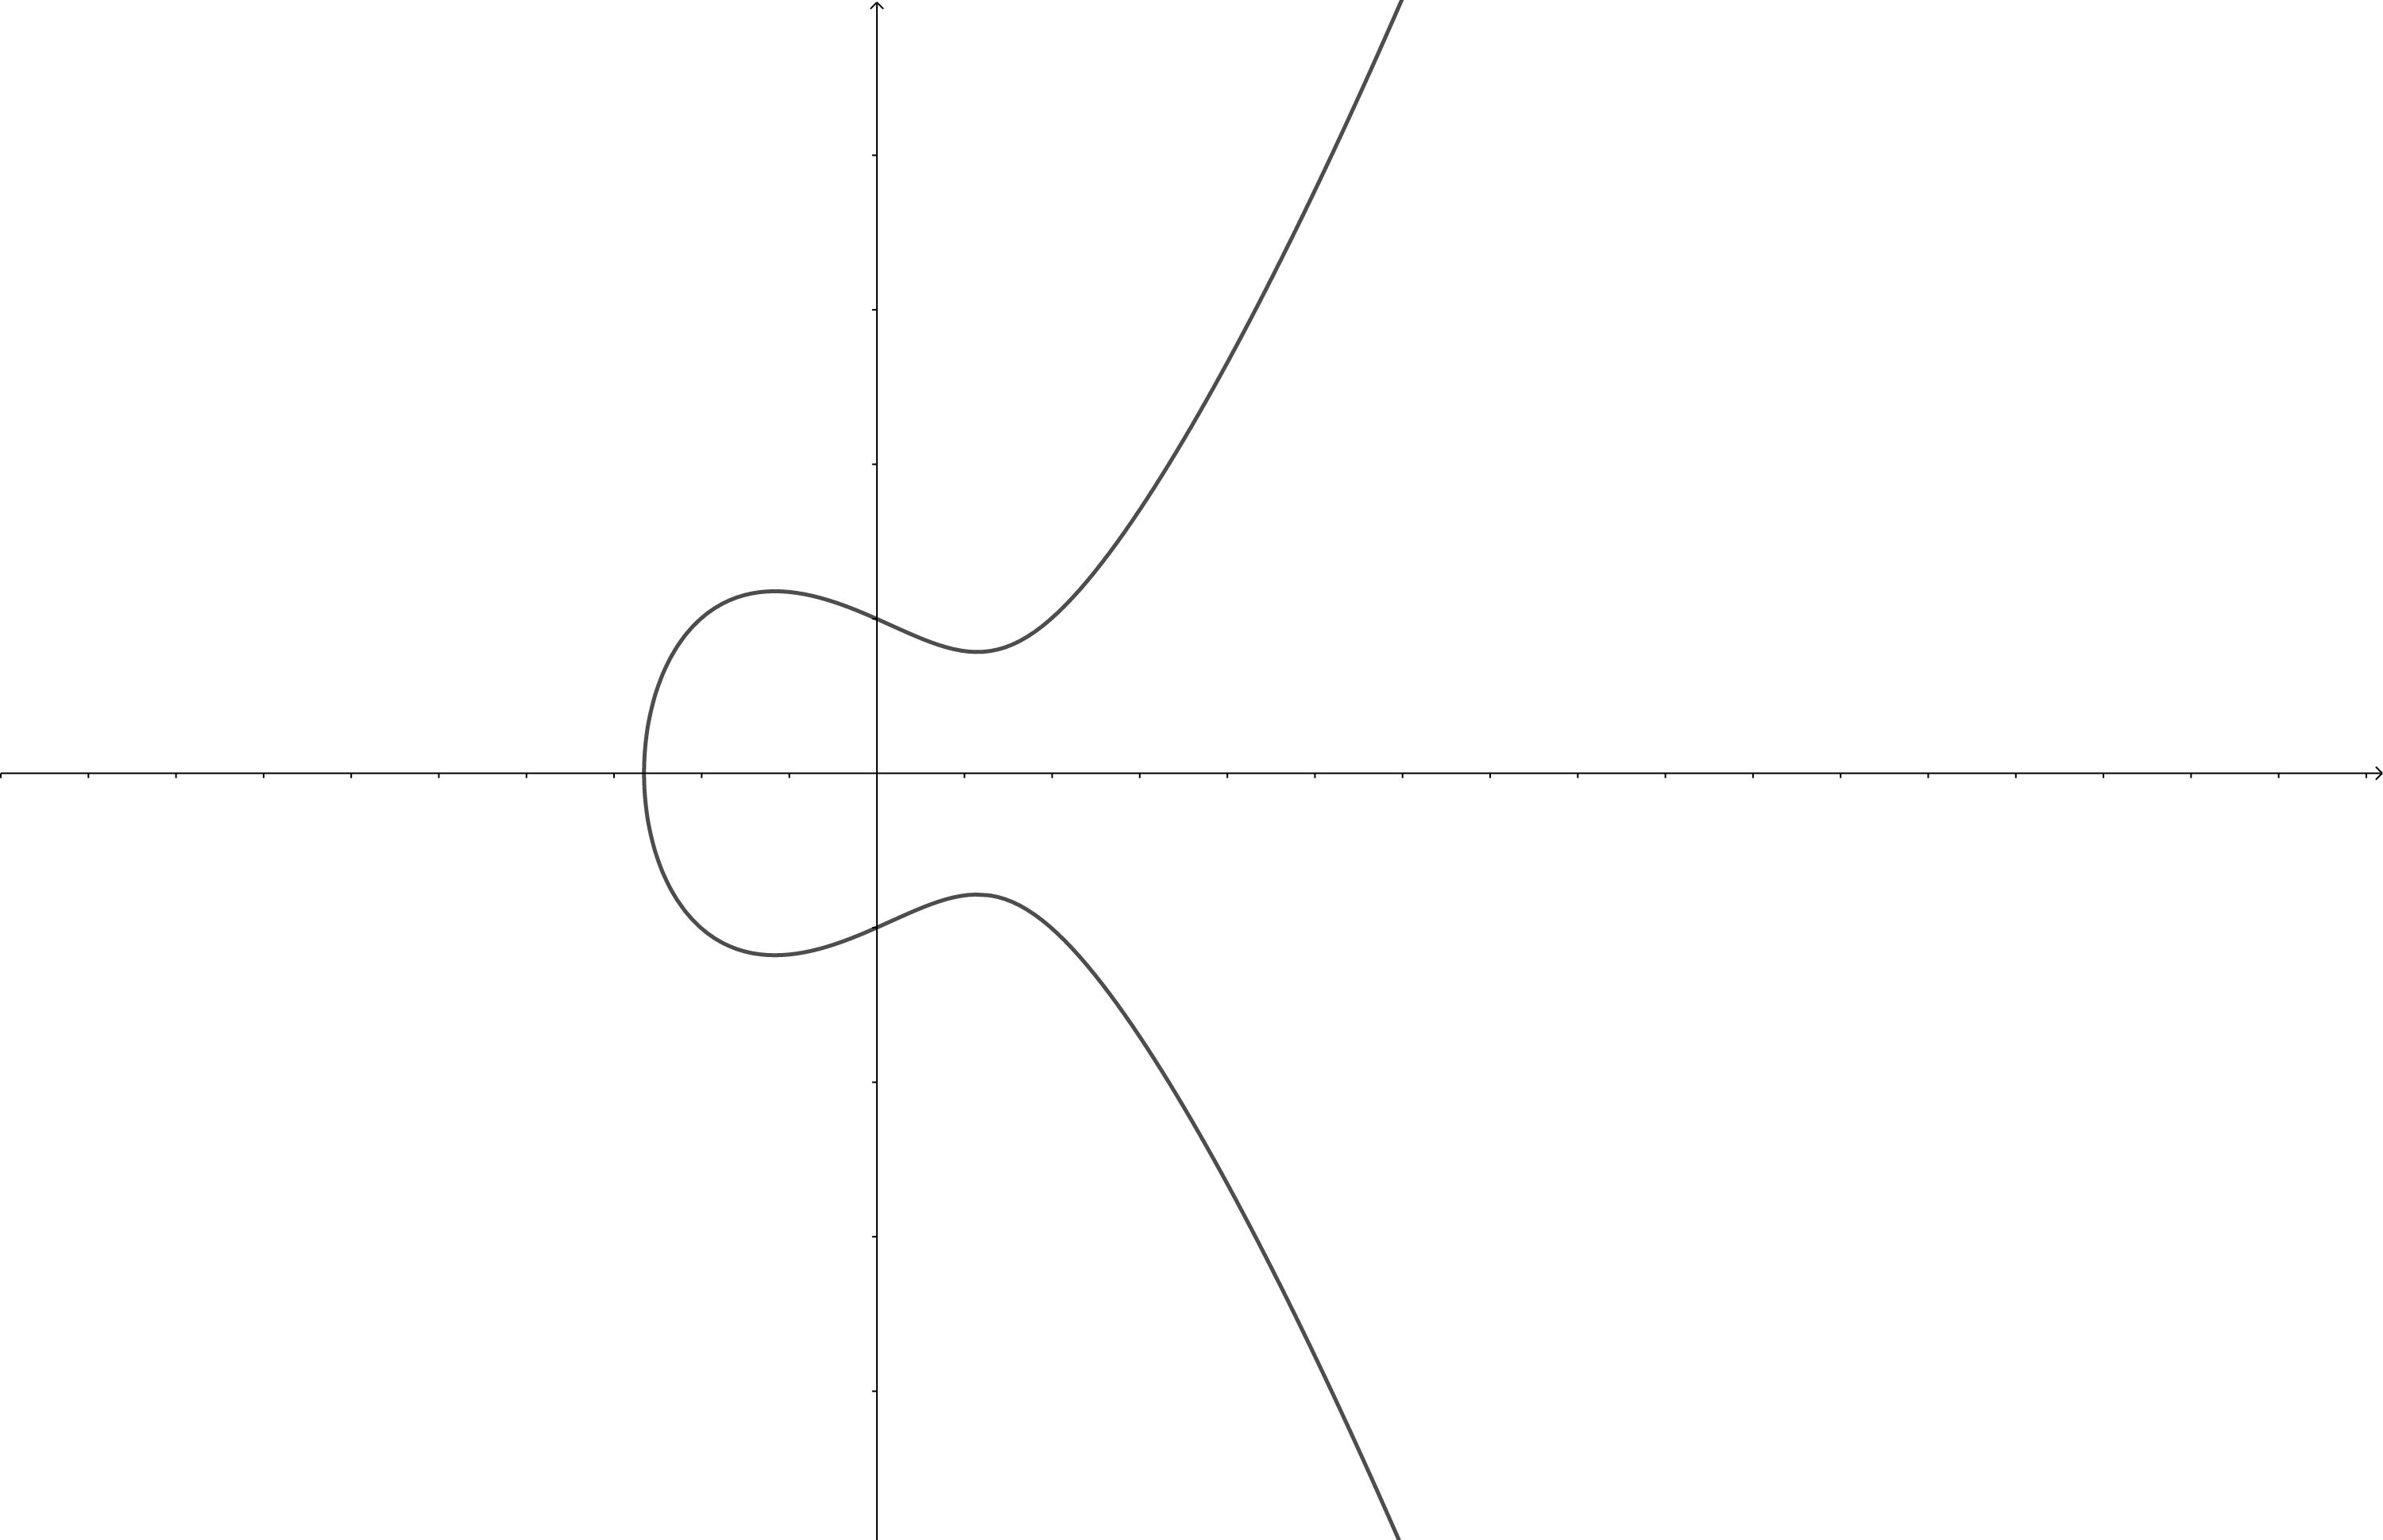
\includegraphics[width=0.4\textwidth]{deltaNeg}
                \caption{Courbe elliptique d'équation $y^2 = x^3 - x + 1$}
                \label{fig:deltaNeg}
            \end{figure}
        \item Si $\Delta > 0$, on a trois racines réels distinctes et donc des courbes
            elliptique de la forme suivante
            \begin{figure}[h]
                \centering
                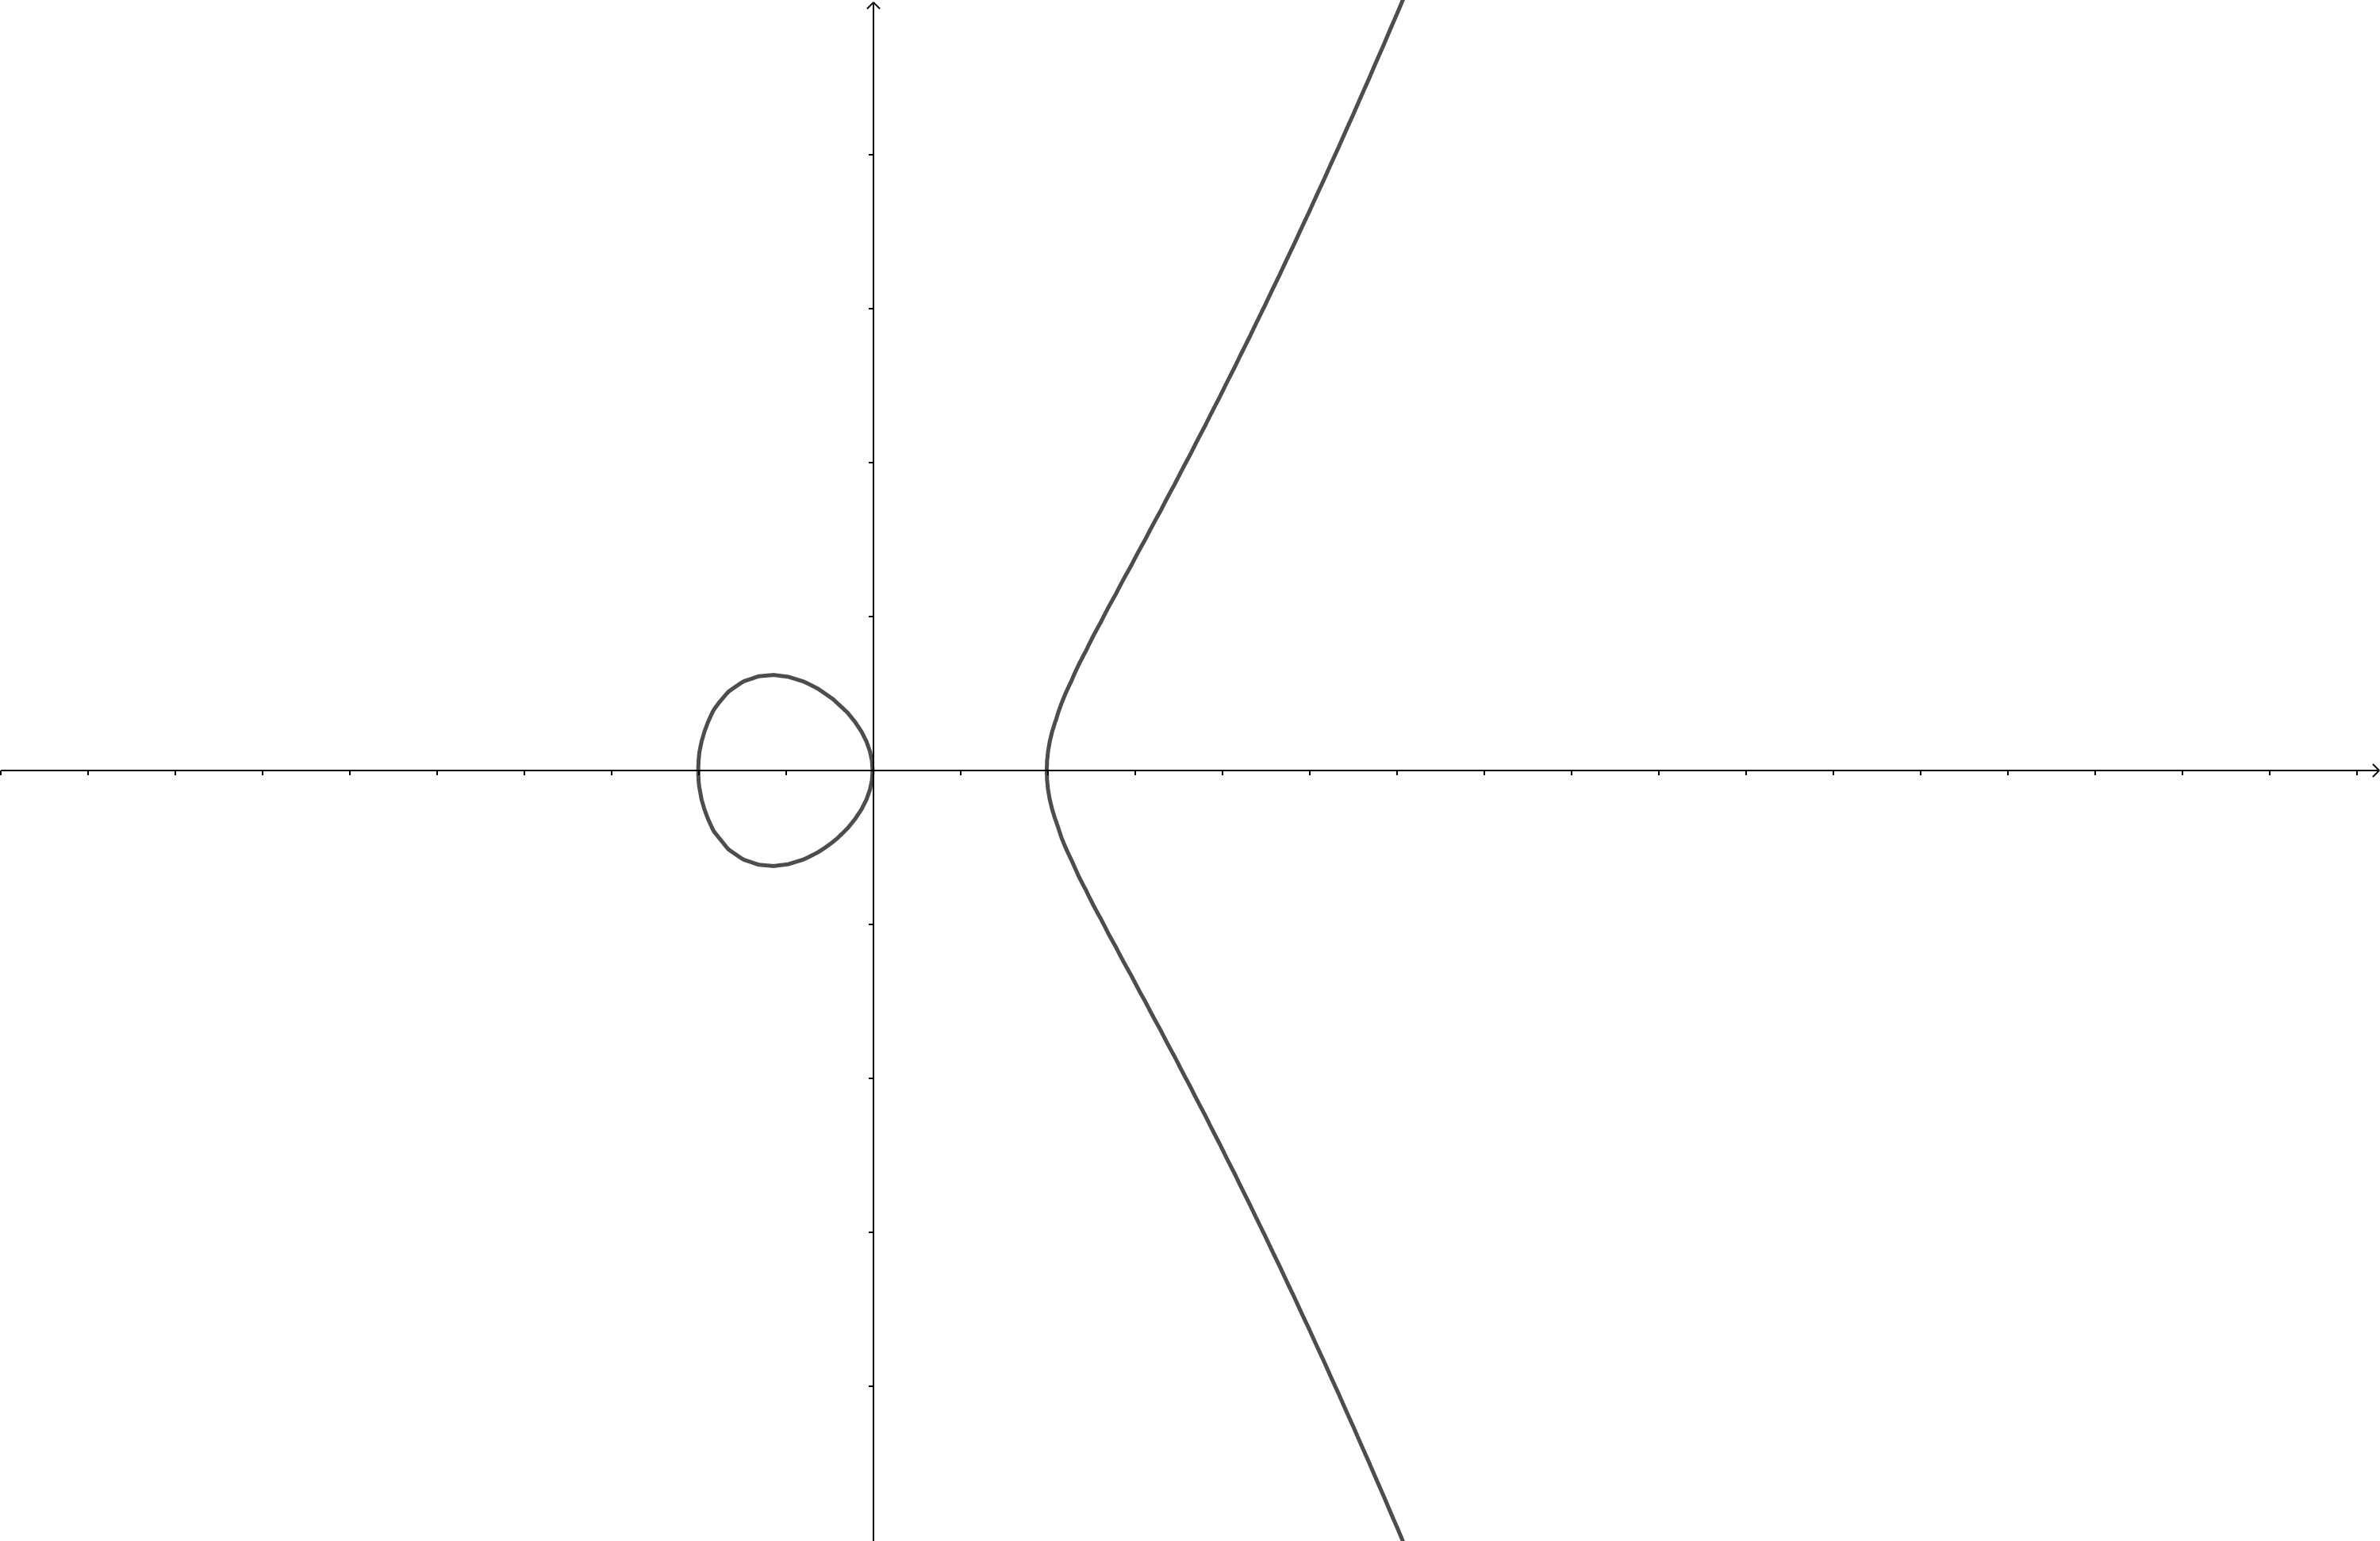
\includegraphics[width=0.4\textwidth]{deltaPos}
                \caption{Courbe elliptique d'équation $y^2 = x^3 - x$.}
                \label{fig:deltaPos}
            \end{figure}

        \item Si $\Delta = 0$ alors la courbe n'est pas elliptique et on obtient un point
            singulier.
            \begin{figure}[h]
                \centering
                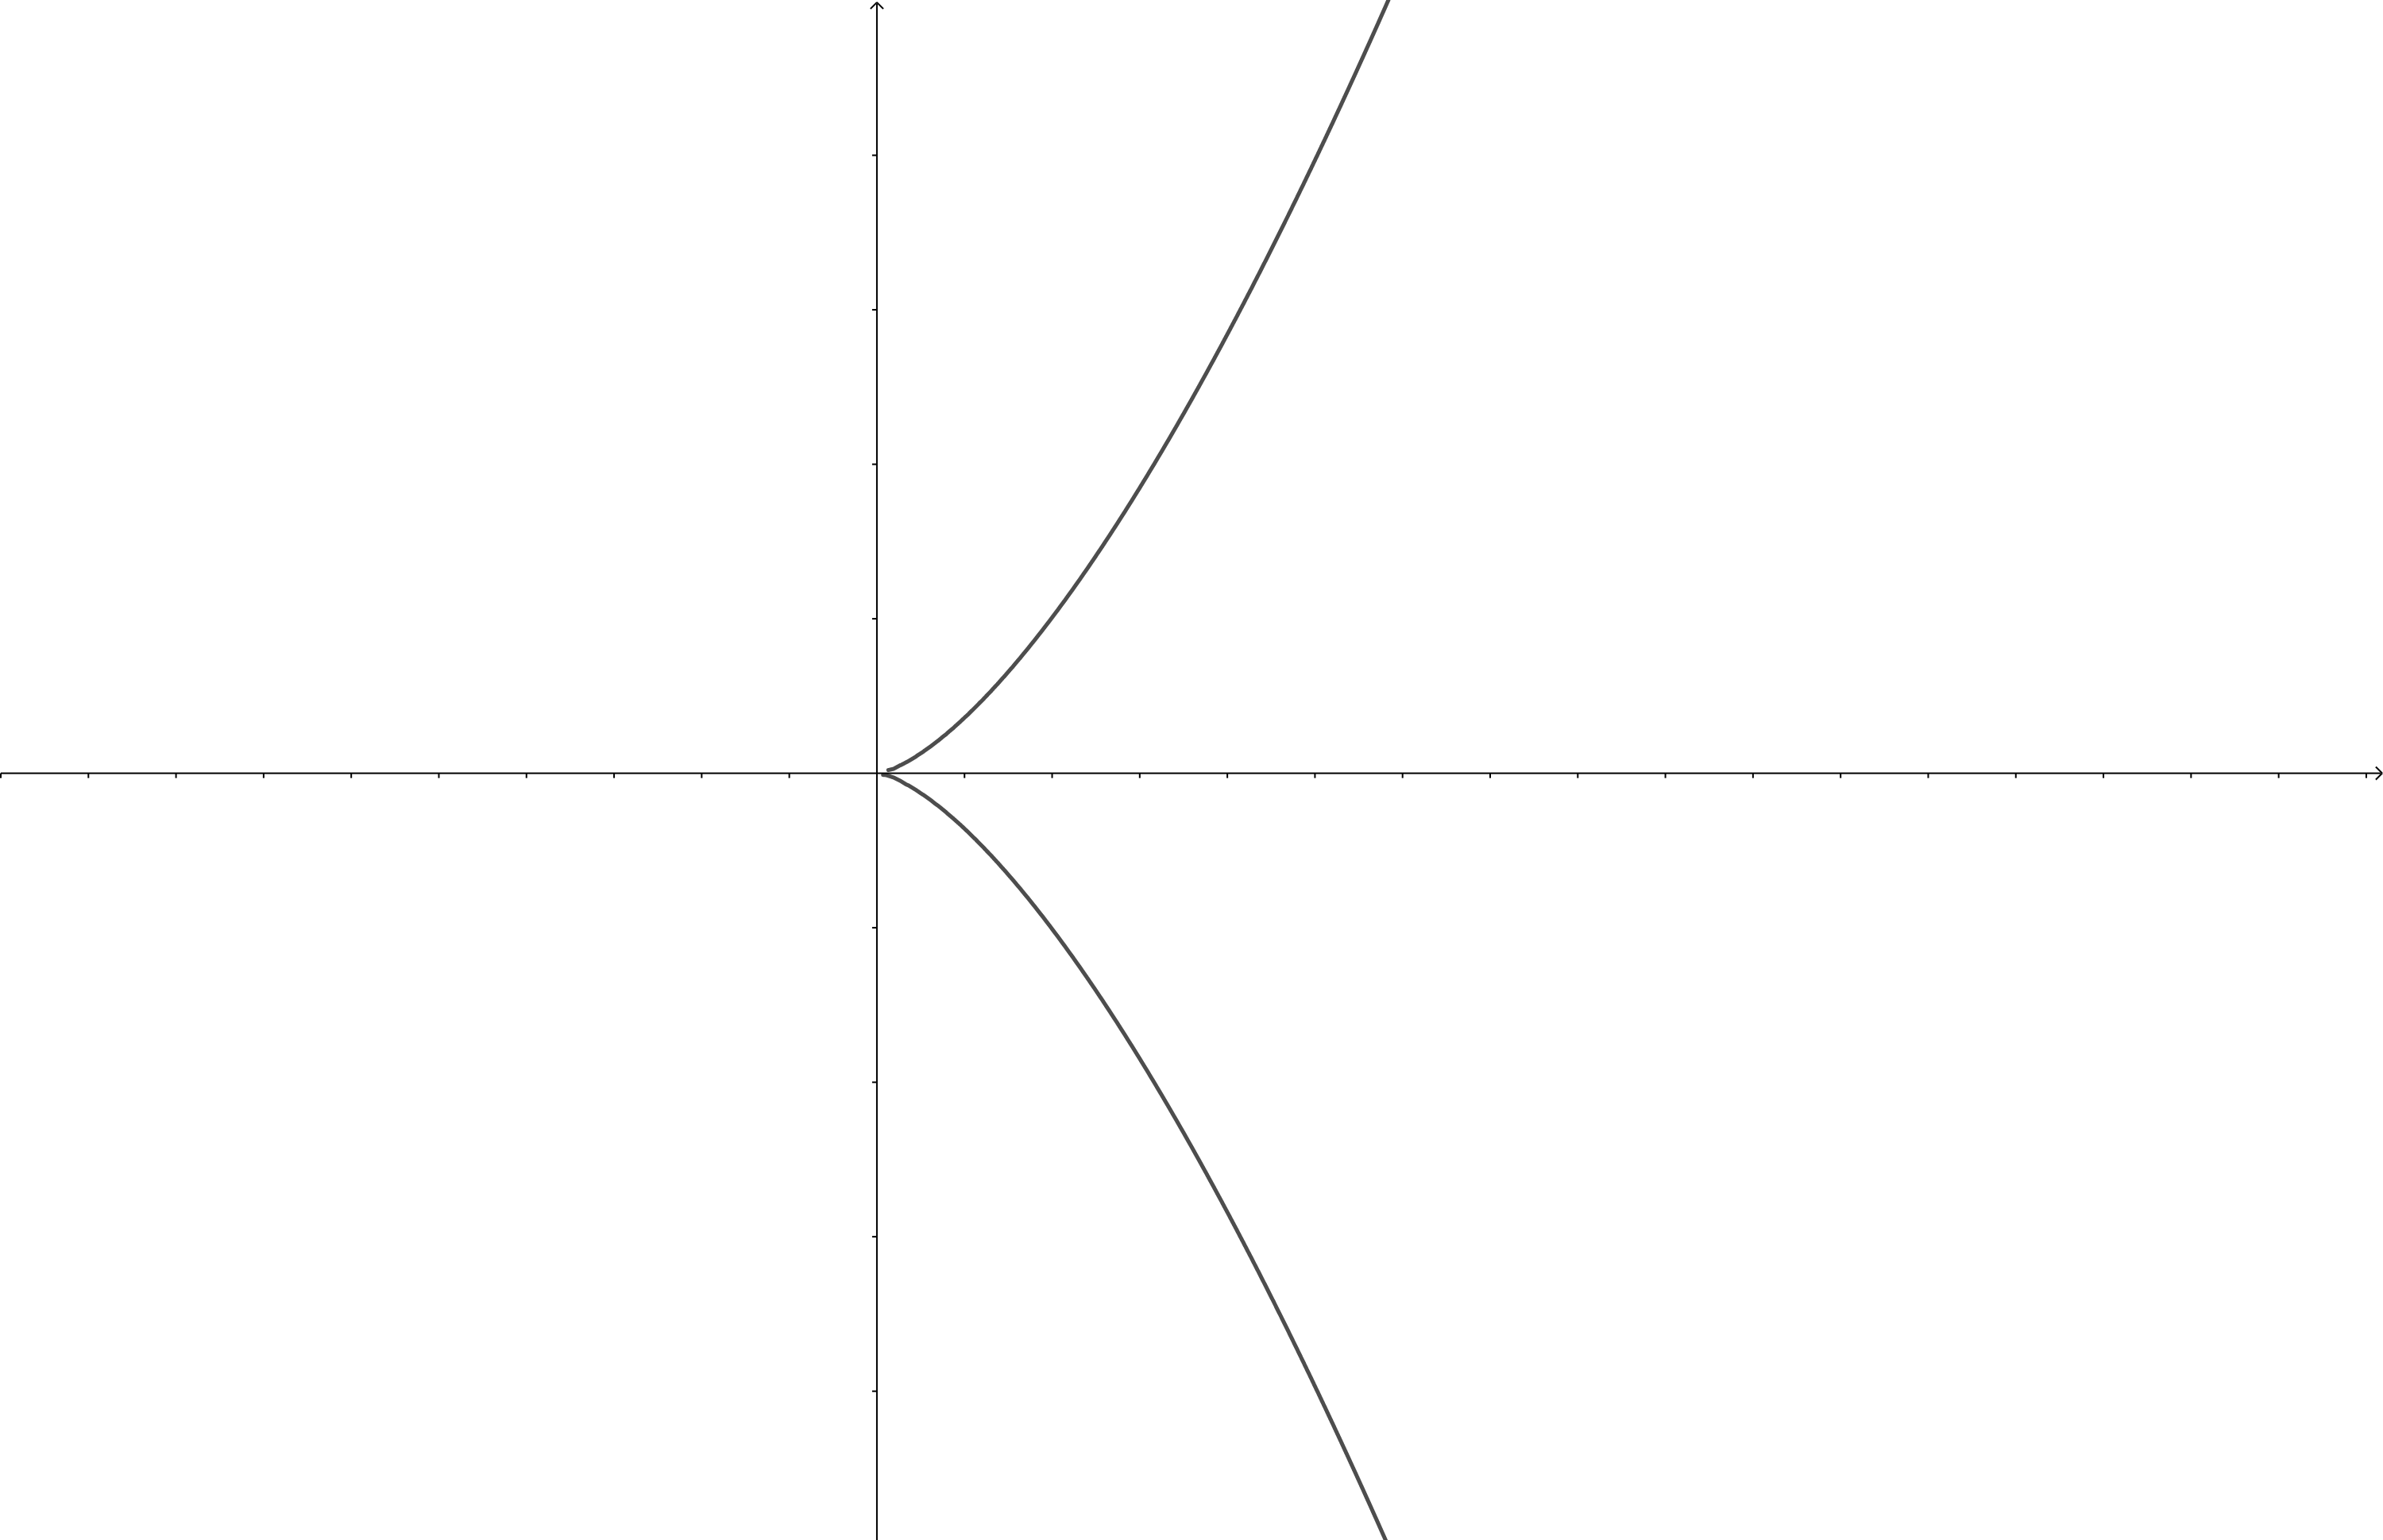
\includegraphics[width=0.4\textwidth]{deltaNul}
                \caption{Courbe elliptique d'équation $y^2 = x^3$.}
                \label{fig:deltaNul}
            \end{figure}
    \end{enumerate}
\end{remarque}

Comme on vient de le voir, il est possible de se ramener à l'étude
des solution de l'équation
polynômial $f(x,y) = 0$ dans le plan affine. Ainsi la condition \eqref{eq:delta}
signifie que les racines dans $\overline{K}$ du polynôme
\[
f(x,y) = y^2 - x^3 + ax + b
,\] 
sont simples et le lemme suivant nous fourni un critère simple pour obtenir une courbe
lisse. Ce qui nous permet d'éviter les courbes avec un point de multiplicité double qui nous
fait perdre l'unicité de la tangente.
\begin{figure}[h]
    \centering
    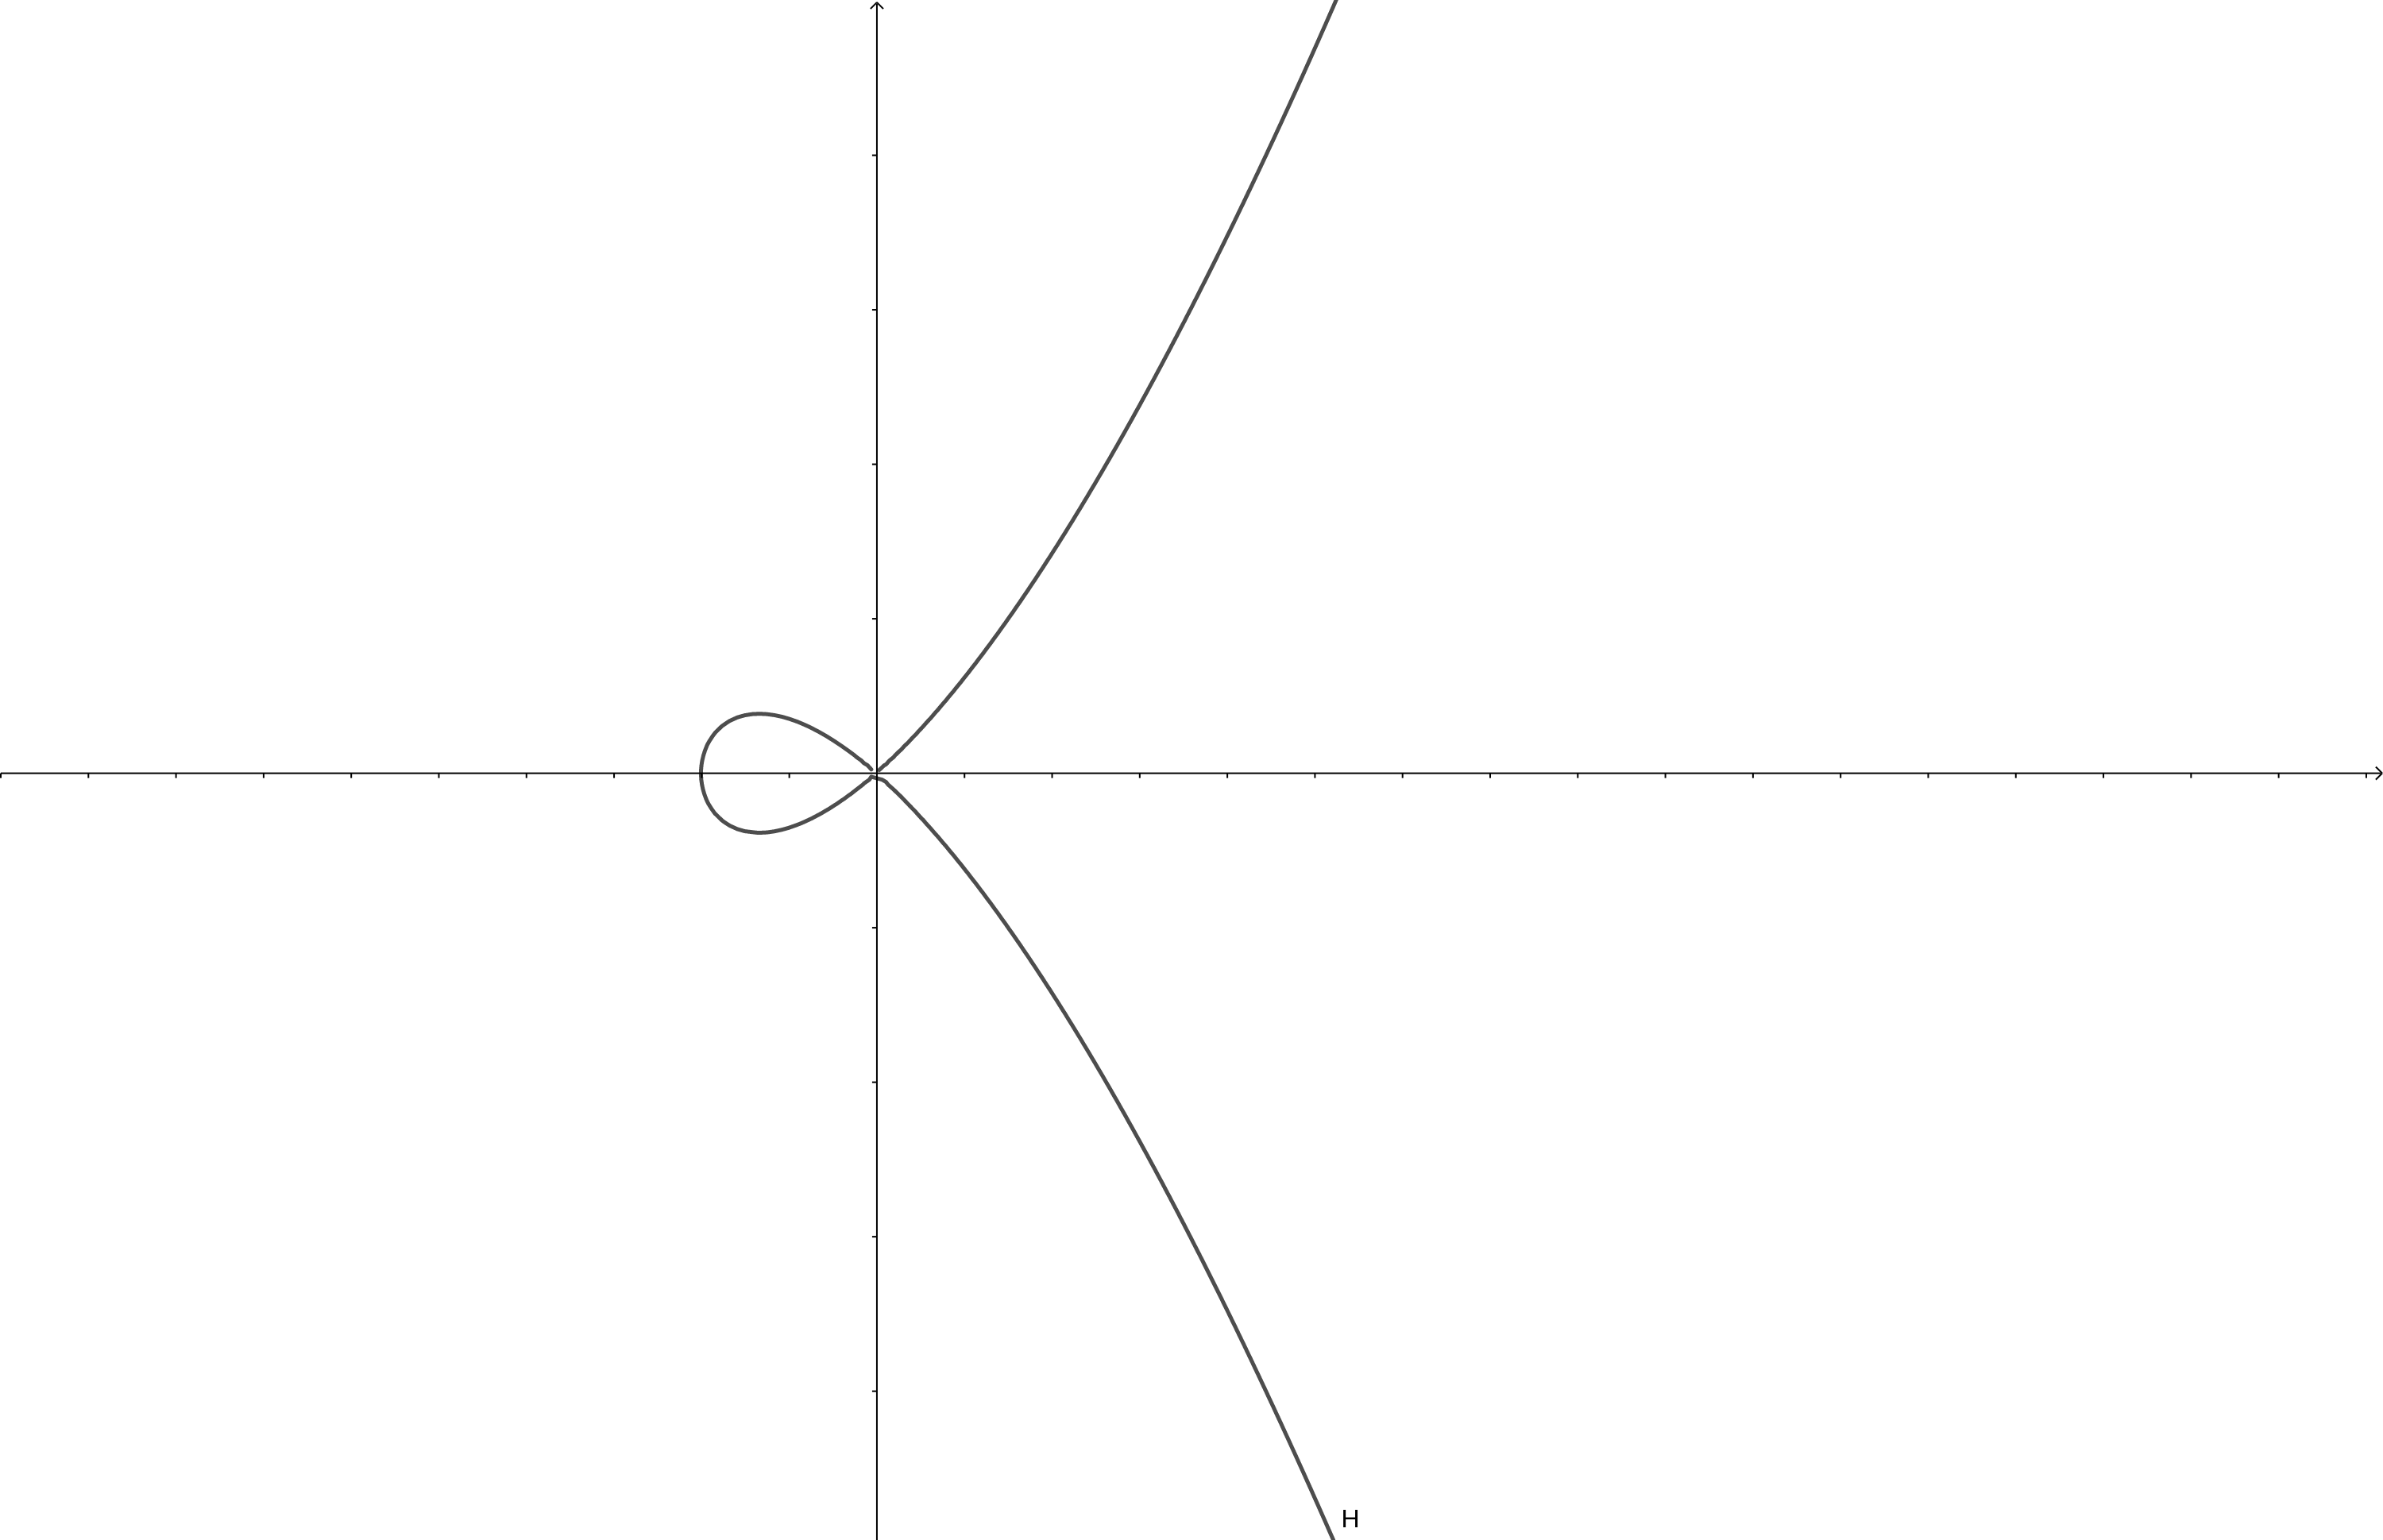
\includegraphics[width=0.5\textwidth]{courbeSing}
    \caption{Courbes d'équation $y^2 = x^3 + x^2$ admettant un point double.}
    \label{fig:courbeSing}
\end{figure}

\begin{lemme}
    \label{lem:lemme1}
    Le discriminant de $f$ est $\Delta = -(4a^3 + 27b^2)$. En particulier, les racines de $f$ sont simples, si et seulement si $\Delta \neq 0$.
\end{lemme}

Pour démontrer ce lemme, on utilise la proposition que nous admettrons, qui est la suivante:
\begin{proposition}
    \label{prop:discriminant}
    Soit $g$ un polynôme unitaire à coefficients dans $K$ de degré $n \ge 1$. Soient
    $\alpha_1,\ldots,\alpha_{n}$ ses racines dans $\overline{K}$ comptées avec
    multiplicités. Le discriminant $\Delta$ de $g$ est défini par l'égalité
    \[
    \Delta = \prod_{i<j}^{} \left( \alpha_{i} - \alpha_{j} \right) ^2 
    .\] 
    C'est un élément de $K$.
\end{proposition}

\begin{demonstration}[Lemme]
    Montrons tout d'abord que le discriminant de $f$ est $\Delta= -(4a^3 + 27b^2)$.

    Soit $\Delta$ le discriminant de $f$. Soient $\alpha, \beta, \gamma $ les racines de $f$ dans $\overline{K}$ et $f'$ le polynôme dérivé de $f$.

    À l'aide de la proposition \ref{prop:discriminant}, on veut montrer que le discriminant est de la forme
    suivante: 
    \begin{align*}
        \Delta &= (-1) ( \alpha - \beta )^2 ( \alpha - \gamma )^2 ( \beta - \gamma )^2 \\
          &= - f(\alpha)'f(\beta )'f(\gamma)'
    .\end{align*}

    Vérifions que c'est bien le cas.

    D'aprés le théorème d'Alembert-Gauss comme $f \in \overline{K}$, on dispose de la
    forme scindé de $f$.
    \[
        f = \left( X - \alpha \right) \left( X - \beta \right) \left( X - \gamma \right) 
    .\] 
    En dérivant $f$ sous cette forme on obtient :
    \begin{align*}
        f &= ( X - \alpha ) \left( ( X - \beta ) ( X - \gamma ) \right)'  + ( X - \beta ) ( X - \gamma )\\
          &= ( X - \alpha ) \left( ( X - \beta ) + ( X - \gamma ) \right) + ( X - \beta ) ( X - \gamma ) 
    .\end{align*}

    Donc  
\[
f' = ( X - \alpha ) ( X - \beta ) + ( X - \alpha ) ( X - \gamma ) + ( X - \beta ) ( X - \gamma )
.\] 

On a alors successivement : 
\[
    f(\alpha)' = ( \alpha - \beta) ( \alpha - \gamma )
,\] 
\[
f(\beta )' = ( \beta - \alpha) ( \beta - \gamma)
,\] 
et
\[
f(\gamma)' = ( \gamma - \alpha) ( \gamma - \beta)
.\] 

En multipliant ces trois expressions, on obtient :
\begin{align*}
    f(\alpha)' f(\beta )' f(\gamma)' &= ( \alpha - \beta ) ( \alpha - \gamma ) ( \beta - \alpha ) ( \beta - \gamma) ( \gamma - \alpha ) ( \gamma - \beta ) \\
&= \left( X - \alpha \right) \left( \alpha - \gamma \right) \left( -1 \right) \left( \alpha - \beta  \right) \left( \beta - \gamma \right) \left( -1 \right) \left( \alpha - \gamma \right) \left( -1 \right) \left( \beta - \gamma \right) \\
&= \left( -1 \right) ^3 \left( \alpha - \beta  \right) ^2 \left( \alpha - \gamma  \right) ^2 \left( \beta - \gamma \right) ^2\\
 &= - \Delta
.\end{align*}

Et donc 

\[
\Delta = - f'(\alpha) f'(\beta ) f'(\gamma)
.\] 

En partant de la forme $f : x^3 + ax + b$, on remarque que $f' : 3x^2 + a$. Par suite on obtient,
\begin{align*}
    \Delta &= - f'(\alpha) f'(\beta ) f'(\gamma) \\
      &= - \left( 3 \alpha^2 + a \right) \left( 3 \beta^2 + a \right) \left( 3 \gamma^2 + a \right) 
.\end{align*}
Ce qui donne :
\begin{align*}
    \Delta  &= - \left( ( 9 \alpha^2 \beta^2 + 3a ( \alpha^2 + \beta^2 ) + a^2 ) ( 3 \gamma^2 + a ) \right)  \\
       &= - \left( 27 \left( \alpha \beta \gamma \right)^2  + 9a \left( \alpha^2 \beta^2 + \alpha^2 \gamma^2 + \beta^2 \gamma^2 \right) + 3a^2 \left( \alpha^2 + \beta^2 + \gamma^2 \right) + a^3 \right) 
.\end{align*}
On peut écrire
\[
\alpha^2 + \beta^2 + \gamma^2 = \left( \alpha + \beta + \gamma \right)^2 - 2 \left( \alpha \beta + \alpha \gamma + \beta \gamma \right)
,\] 
\[
\alpha^2 \beta^2 + \alpha^2 \gamma^2 + \beta^2 \gamma^2 = \left( \alpha \beta + \alpha \gamma + \beta \gamma \right)^2 - 2\alpha \beta \gamma \left( \alpha + \beta + \gamma \right)
.\] 
Donc d'après les relations entre coefficients et racine (i.e relation de Viète), pour un polynôme de la forme $ax^3 + bx^2 + cx + d$, on a :
\[
\alpha + \beta + \gamma = - \frac{b}{a}
,\] 
\[
\alpha \beta + \alpha \gamma + \beta \gamma = \frac{c}{a}
,\] 
\[
\alpha \beta \gamma = - \frac{d}{a}
.\] 
Ici dans $f$ on a $a = 1$, $b = 0$, $c = a$ et $d = b$.

D'où,
\[
\alpha + \beta + \gamma = 0 \text{, } \alpha \beta + \alpha \gamma + \beta \gamma = a \text{ et } \alpha \beta \gamma = - b
.\] 
Ce qui donne : 
\begin{align*}
    \alpha^2 + \beta^2 + \gamma^2 &= 0^2 - 2a = -2a \\
    \alpha^2 \beta^2 + \alpha^2 \gamma^2 + \beta^2 \gamma^2 &= a^2 + 2b \times 0
.\end{align*}

Donc le discriminant vaut :
\begin{align*}
    \Delta &= - \left( 27b^2 + 9a^3 - 6a^3 + a^3  \right) \\
        &= - \left( 4a^3 + 27b^2  \right)
.\end{align*}

Montrons maitenant que les racines de $f$ sont simple, si et seulement si, $\Delta \neq 0$

Raisonnons par contraposition et montrons que les racine de $f$ sont multiples, si et
seulement si, $\Delta = 0$. 

Supposons que $\Delta = 0$. On a alors :
 \begin{align*}
     - \left( 4a^3 + 27^2 \right) = 0 &\iff - f(\alpha)' f(\beta )' f(\gamma)' = 0 \\
                                      & \iff \left( f(\alpha)' = 0 \right) \ou \left( f(\beta )' = 0 \right) \ou \left( f(\gamma)' = 0 \right) \\
                                      &\iff \alpha \text{ ou } \beta \text{ ou } \gamma \text{ est une racine multiple}
.\end{align*}

D'où le résultat.
\end{demonstration}

% \section{Partie affine et point à l'infini}

% Dans cette section nous définissons explicitement ce que nous avons pu décrire au préalable
% dans la section \ref{defGene} 

% Considérons des éléments $a$ et $b$ de $K$ tels que $4a^3+27b^2 \neq 0$. Soit $E$ la courbe
% elliptique d'équation homogène
% \[
% E :\quad y^2z=x^3+axz^2+bz^3
% .\] 

% Soit $U = \left\{ [x,y,z] \in \mathbb{P}_{2} \mid z \neq 0 \right\} $. On a vu qu'a l'aide
% d'une application $\phi$, on obtient une bijection entre le plan affine et l'ensemble $U$.

% Par ailleurs, $E \cap U$ s'identifie via $\phi$ à l'ensemble des éléments $(x,y)$ de $\overline{K}^2$ vérifiant l'égalité

% \begin{align}
%     \label{eq:ell1}
% y^2 = x^3 + ax + b
% .\end{align}

% On dira que $E \cap U$ est la partie affine de $E$ et que $O$ est le point à la l'infini de $E$.

% Dans toute la suite, on identifira $E \cap U$ et le sous-ensemble de $\overline{K}^2$ formé des éléments $(x,y)$ vérifiant \eqref{eq:ell1}. Avec cette identification, on a 
% \[
% E = \left\{ (x,y) \in \overline{K} \times \overline{K} \mid y^2=x^3+ax+b \right\} \cup \left\{ O \right\} 
% .\] 

% Ainsi, $E$ est la courbe affine d'équation \eqref{eq:ell1} à laquelle on adjoint le point à l'infini $O$. C'est pourquoi on définira souvent une courbe elliptique par sa partie affine, sans préciser le point $O$.

% \begin{remarque}
%     On retiendra qu'une courbe affine d'équation de la forme \eqref{eq:ell1} est une courbe
%     elliptique si et seulement si, par définition, la condition \eqref{eq:delta} est satisfaite.
% \end{remarque}



% Comme par définition, c'est une courbe sur le plan projectif, on dispose du polynôme homogène
% de degré $3$, $F(X,Y,Z)$ dans l'anneau de polynôme $K[X,Y,Z]$. Étant données $ a,b \in K$. 

% Posons 
% \[
% F=Y^2Z-\left( X^3+aXZ^2+bZ^3 \right) 
% .\] 

% Comme $F$ est homogène de degré $3$. Par la définition \eqref{def:courbe}, on a donc
% $E$ la courbe sur le plan projectif $\mathbb{P}_{2}$ qui est l'ensemble des solutions de l'équation
% polynômiale
% \[
% E: \quad F(X,Y,Z) = 0
% ,\] 
% Si $\left( x,y,z \right) $ est un éléments non nul de $\overline{K}^3$, cette condition
% ne dépend que de sa classe dans $\mathbb{P}_{2}(\overline{K})$.

% Soit $P = \left[ x,y,z \right] $ un point de $\mathbb{P}^2(\overline{K})$. On
% dit que $P$ est un zéro de $F$ dans $\overline{K}$, ou plus simplement un zéro de $F$, si
% l'on a $F(x,y,z)=0$. On signifie par, courbe projective plane d'équation \eqref{eq:ell},
% l'ensemble des zéros de $F$ dans $\overline{K}$.

% Quant à la condition \eqref{eq:delta}, elle signifie que les racines dans $\overline{K}$ du
% polynôme
% \[
% f = X^3 + aX + b
% \] 
% sont simples.



% \begin{remarque}
% \end{remarque}


\section{Points rationnels d'une courbe elliptique}

Soit $L$ une extension de $K$ dans $\overline{K}$.

\begin{definition}
    Soit $P=\left[ x,y,z \right] $ un point de $\mathbb{P}^2$. On dit que $P$ est rationnel sur $L$ s'il existe $\lambda \in \overline{K}^{*}$ tel que $\lambda x$, $\lambda y$ et $\lambda z$ soient dans $L$. On note $\mathbb{P}^2(L)$ l'ensemble des points de $\mathbb{P}^2$ rationnels sur $L$.

\end{definition}

D'aprés la définition ci-dessus, un point non nul $P$ est dans $\mathbb{P}_{2}(L)$, si sa classe est dans $L$. Autrement
dit, 
\[
\mathbb{P}_{2}(L)=\left\{ P \in \overline{K}^{3} \mid \exists \lambda \in \overline{K}^{*}, P =
\lambda P\right\} 
.\] 

Cela justifie la notation $\mathbb{P}^2 = \mathbb{P}^2(\overline{K})$.

\begin{remarque}
    Étant donné un point $[x_1,x_2,x_3] \in \mathbb{P}^2$, le fait qu'il soit rationnel sur $L$ n'implique pas que les $x_{i}$ soient dans $L$. Cela signifie qu'il existe $i$ tel que $x_{i}$ soit non nul, et que chaque $\frac{x_{j}}{x_{i}}$ appartienne à $L$.

    En effet, soit un point $P \in \mathbb{P}_{2}$ non nul. Si $P \in \mathbb{P}_{2}(L)$,
    comme il est non nul, il existe $x \neq 0$, et pour $\lambda = x$, on a $P =
    [1,\frac{y}{x},\frac{z}{x}]$ et on a bien $\frac{y}{x},\frac{z}{x} \in L$ et pourtant ce
    sont des variables indéterminées de $\overline{K}$.
\end{remarque}

Soit $E$ une courbe elliptique définie sur $K$ d'équation \eqref{eq:ell}.

\begin{definition}
    Un point de $E$ est dit rationnel sur $L$, ou encore $L$-rationnel, s'il appartient à $E \cap \mathbb{P}^2(L)$. On note $E(L)$ l'ensemble des points de $E$ rationnels sur $L$.
\end{definition}

Par définition, on a donc
\[
E = E(\overline{K})
.\] 

% Le point $O = [0,1,0]$ appartient à $E(K)$. Soit $(x,y) \in \overline{K}^2$ un point de la partie affine de $E$. Par définition, il est rationnel sur $L$ si et seulement si $x$ et $y$ sont dans $L$. Il en résulte que l'on a 
% \[
% E = \left\{ (x,y) \in L \times L \mid y^2 = x^3+ax+b \right\} \cup \left\{ O \right\} 
% .\] 


\begin{remarque}
    \begin{enumerate}
        \item  Lorsque le contexte est clair on parlera de point rationnel de la courbe pour
            parler des points $L$-rationnels.
        \item Le point $\mathcal{O}$ est défini sur $K$ et par définition sur toute
            extension de $K$. Ainsi, si $L / K$ est une extension du corps $K$, $E$
            peut-être considérée comme une courbe elliptique définie sur $K$ et $\mathcal{O}$
            est encore le point à l'infini de $E / L$.

            On a,

            \[
            E(L) = \left\{ (x,y) \in L^2 \mid y^2 = x^3 + ax + b \right\} \cup {\mathbb{O}}
            .\] 

            De même,
            \[
            E(\overline{K}) = \left\{ (x,y) \in \overline{K}^2 \mid y^2 = x^3 +
            ax + b \right\} \cup {\mathbb{O}}
            .\] 

            Ce qui revient à dire que, si $K \subset L \subset \overline{K}$ alors $E(K)
            \subset E(L) \subset E(\overline{K})$.
    \end{enumerate}
\end{remarque}

\begin{exemple}
    Soit la courbe $E$ définie sur $\mathbb{F}_{5}$ d'équation
    \[
    y^2 =x^3+x+1
    .\] 

    Cette courbe vérifie bien la condition \eqref{eq:delta}.
    
    En effet, on a $\Delta = -(4 \times 1^3 + 27 \times 1) = -31$.

    L'ensemble des points de la courbe est le suivant:
    \[
    E(\mathbb{F}_{5})= \left\{ (0,1),(0,4),(2,1),(2,4),(3,1),(3,4),(4,2),(4,3) \right\} \cup
    \left\{ \mathcal{O} \right\} 
    .\] 

    \textbf{exemple klaus F25}
    % En effet, comme la courbe est symétrique, il nous suffit de vérifier que pour tous les
    % valeurs de $x$ dans $\mathbb{F}_{5}$, lesquelles sont un carré dans $\mathbb{F}_{5}$.

    % Par exemple, pour $x=0$, on a $y^2=0^3+0+1$ donc $y = \pm 1$, ce qui nous donne
    % les points d'abiscisse $x=0$ et d'ordonnées $y=\pm 1$ dans $\mathbb{F}_{5}$, par
    % conséquent les points $(0,1)$ et $(0,4)$ vérifient l'équation $f(x,y) = 0$ et sont
    % donc des points de la courbe.

    % Maintenant si $x=1$, l'équation de la courbe nous donne $y^2=1^3+1+1=3$ donc il faut
    % chercher si dans $\mathbb{F}_{5}$, s'il existe un carré modulo $5$ égal à 3. Ce qui n'est
    % pas le cas. En effet, dans $\mathbb{F}_{5}$ les éléments sont $\left\{
    % \overline{0},\overline{1},\overline{2},\overline{3},\overline{4} \right\} $ et on a
    % succecssivement dans $\mathbb{F}_{5}$
    % \begin{align*}
    %     y^2 &=0^2=0 \\
    %     y^2 &= 1^2 = \pm 1 \\
    %     y^2 &= 2^2=4=-1 \\
    %     y^2 &= 3^2=9=-1 \\
    %     y^2 &= 4^2=16=1 \\
    % .\end{align*}
    % Ainsi, il n'existe pas $y \in \mathbb{F}_{5}$ qui vérifient l'équation de la
    % courbe. Donc la courbe $E$ ne possède pas de point de d'abscisse $x=1$.

    % À voir si je mets $\mathbb{F}_{25}$ je crois j'ai pigé faut que je vérifie ça ce midi
\end{exemple}
